\subsection{Controlled HTTP/2 comparisons}
\begin{table*}[t]\centering\small
\begin{tabular}{llrrrrrrr}\toprule
Workload / trial & Policy & Replay (s) & Output tok/s & Mean (s) & p95 (s) & Rollout (s) & KV hit & Retries\\\midrule
Warmed reuse 1 & KV+P & 289.1 & 2721 & 30.1 & 56.4 & 46.7 & 0.940 & 0 \\
Warmed reuse 1 & Domains+P & 275.9 & 2851 & 29.9 & 58.0 & 43.5 & 0.953 & 0 \\
Warmed reuse 2 & KV+P & 289.8 & 2714 & 33.3 & 61.0 & 48.2 & 0.930 & 0 \\
Warmed reuse 2 & Domains+P & 284.7 & 2762 & 31.0 & 61.7 & 43.2 & 0.963 & 0 \\
Version turnover 1 & KV+P & 355.9 & 3130 & 39.2 & 81.6 & 51.8 & 0.955 & 0 \\
Version turnover 1 & Domains+P & 350.8 & 3176 & 28.8 & 61.3 & 37.7 & 0.970 & 0 \\
Version turnover 2 & KV+P & 354.8 & 3140 & 39.3 & 81.0 & 49.6 & 0.956 & 0 \\
Version turnover 2 & Domains+P & 365.0 & 3052 & 31.0 & 58.9 & 39.0 & 0.965 & 0 \\
Dialogue 1 & KV+P & 376.8 & 3130 & 18.5 & 49.8 & 90.5 & 0.951 & 0 \\
Dialogue 1 & Domains+P & 316.9 & 3722 & 21.4 & 43.8 & 78.8 & 0.905 & 0 \\
Dialogue 2 & KV+P & 362.1 & 3257 & 18.7 & 50.4 & 87.5 & 0.950 & 0 \\
Dialogue 2 & Domains+P & 295.7 & 3989 & 20.5 & 38.3 & 79.6 & 0.916 & 0 \\
64 versions 1 & KV & 440.5 & 2381 & 60.1 & 237.6 & -- & 0.654 & 0 \\
64 versions 1 & Domains & 270.6 & 3875 & 53.9 & 113.4 & -- & 0.542 & 0 \\
64 versions 1 & Default & 544.2 & 1927 & 111.3 & 200.7 & -- & 0.053 & 0 \\
64 versions 2 & KV & 427.1 & 2455 & 61.1 & 245.2 & -- & 0.649 & 0 \\
64 versions 2 & Domains & 268.5 & 3906 & 53.8 & 116.0 & -- & 0.548 & 0 \\
Long 512 & KV+P & 415.9 & 4491 & 71.3 & 155.5 & 99.0 & 0.970 & 0 \\
Long 512 & Domains+P & 393.4 & 5414 & 62.2 & 137.5 & 81.3 & 0.956 & 0 \\
Long 1,024 & KV+P & 335.0 & 5674 & 106.0 & 200.9 & 138.2 & 0.971 & 0 \\
Long 1,024 & Domains+P & 261.6 & 6011 & 113.8 & 217.9 & 150.8 & 0.952 & 0 \\
\bottomrule\end{tabular}
\caption{Completed HTTP/2 comparisons, reported separately by trial. All times include any cohort preparation. Replay throughput includes recorded update waits for RL workloads; rollout latency excludes those waits. Trial 2 reverses policy order. No confidence interval is inferred from individual requests.}\label{tab:primary}
\end{table*}

Table~\ref{tab:primary} reports each completed trial separately. The time-series
and latency distributions use the first trial, while the repeat reverses policy
order. The paired ranges below describe these executions, rather than confidence
intervals inferred from individual requests.
The primary comparisons comprise 58,368 logical requests across 17 arms,
including the single default-policy control. All finish without retries; every
arm exceeds 288 observed active pool inputs, and every RL arm exhibits overlap
between different clients' rollout rounds.

\paragraph{Working-set pressure with 64 versions.}
Across the two order-reversed trials, Domains improves useful throughput by
59.1--62.8\%, lowers mean request latency by 10.4--11.9\%, and lowers p95 by
52.3--52.7\% relative to KV (Figure~\ref{fig:general-summary}). GPU loads fall
85.5--89.1\%. Each arm completes the same 2,048 requests without retries.
The repeat runs Domains before KV; the conclusion is not specific to which
policy runs first.

In the first corrected general-serving trial, Domains increases throughput
from KV affinity's 2,381 to 3,875 output tokens/s (62.8\%). Mean request latency
falls from 60.1 to 53.9\,s (10.4\%), and p95 falls from 237.6 to 113.4\,s
(52.3\%). Makespan falls from 440.5 to 270.6\,s. Both arms complete the same
2,048 requests with no retries and reach 512 active requests. Default routing
achieves 1,927 tokens/s, so KV affinity is already a substantially stronger
baseline than the default path.

GPU adapter loads fall from 1,168 to 169 (85.5\%) and evictions from 1,160 to
161. First-prefill hot-adapter admissions rise from 984 of 2,048 (48.0\%) to
1,864 (91.0\%). This does not come from higher prefix reuse: KV hit ratio falls
from .654 to .542, increasing uncached input by 32.3\%. The result demonstrates
a case where maximizing prefix hits is the wrong pool objective.

The aggregate KV ratio includes initially cold requests. In the first trial,
KV affinity's ratios by stream request index are 9.5\%, 77.6\%, 87.2\%, and
87.3\%. Only 7,168 of 8,192 input tokens are shared, so the last two indices
approach the workload's 87.5\% reusable fraction. The 65.4\% aggregate is not
evidence that all later affinity requests miss their prefixes. Domains' later
indices achieve 70.8\%, 72.1\%, and 72.6\%, exposing a real locality sacrifice.

Across the complete trial, an adapter version visits 3.28 replicas on average
under KV, close to the idealized four-key occupancy calculation, versus 1.41
under Domains. A prefix group visits 1.00 versus 1.11 replicas. Thus the router
primarily co-locates different conversations using the same adapter while
allowing some individual prefixes to move. Default routing visits 7.83 replicas
per adapter and 5.16 per prefix group. These are whole-trial destination counts,
distinct from simultaneous residency or active working-set measurements.

During busy observations, the mean active adapter working set per replica falls
from 22.9 to 9.3; the fraction of replica observations exceeding eight active
adapters falls from 98.7\% to 57.3\%. The mean engine-reported running count when
requests are queued rises from 16.3 to 27.5. Both policies keep every replica
nonempty during the sampled busy intervals. Thus the difference is not simply
eliminating entirely idle hosts. Smaller adapter working sets and larger running
batches accompany the throughput gain, despite additional prefill.

These observations are consistent with improved batch compatibility under the
eight-adapter admission limit. The pinned scheduler explicitly skips requests
whose adapter cannot join the running set~\cite{sglang-admission}. We do not
trace every such rejection, so the measurements do not isolate its contribution
from prefill scheduling and queue placement. Summed host elapsed loading time
falls from 86.24 to 11.01\,s;
it is not a decomposition of the 169.9\,s makespan reduction. The domain policy
still exceeds eight active adapters in some observations, as permitted by its
cache-preserving and congestion-escape rules.

The repeat also preserves the mechanism measurements. Mean busy adapter working
sets are 23.5 for KV and 8.5 for Domains; running counts while queued are 16.1
and 28.3. GPU loads are 1,234 versus 135, and hot-adapter admission ratios are
44.9\% versus 93.8\%. KV reuse falls from 64.9\% to 54.8\%. These observations
reinforce the distinction between optimizing a cache-hit metric and improving
pool completion time.

\begin{figure*}[t]\centering
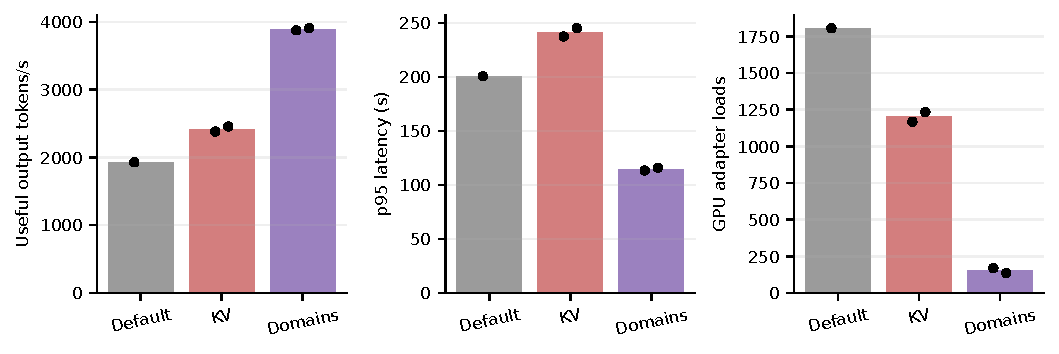
\includegraphics[width=\textwidth]{figures/general-serving.pdf}
\caption{General serving with 64 versions. Points show individual trials; bars
show their arithmetic mean, not a fitted expectation. KV and Domains have two
order-reversed trials; Default has one. All use the corrected eight-connection
HTTP/2 topology and identical requested work.}
\label{fig:general-summary}\end{figure*}

\begin{figure*}[t]\centering
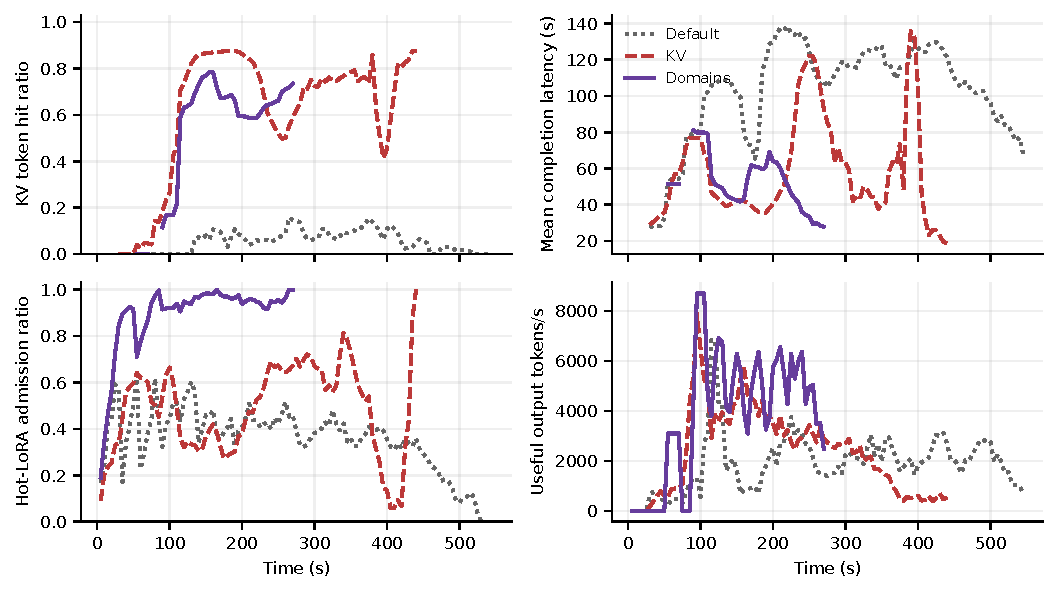
\includegraphics[width=\textwidth]{figures/general-time-series.pdf}
\caption{First corrected 64-version serving trial: 512 independent streams,
8,192-token inputs, and 512-token outputs. Domains sustains more hot-adapter
admissions while accepting fewer KV hits. The same completion-window and
counter-difference definitions as Figure~\ref{fig:timeseries} apply.}
\label{fig:general}\end{figure*}

\paragraph{Warmed reuse.}
Across the two order-reversed trials, Domains+P reduces GPU adapter loads by
43.6--52.0\% and improves replay throughput by 1.8--4.8\%. Mean rollout latency
falls 6.8--10.4\%, while eleven of sixteen clients improve in each trial.
The p95 request latency nevertheless rises 1.2--2.7\% in both trials.
Avoiding adapter movement is repeatable here, but the end-to-end throughput
benefit is much smaller than in the 64-version workload.

The requested-token KV ratio rises in both trials. Its relationship to actual
prefill work is less consistent: seed-inclusive uncached input rises from
13.4\% to 14.5\% of logical input in the first trial, but falls from 14.9\% to
13.6\% in the repeat. Each arm issues 384 seeds. Counting those seeds' uncached
input is necessary to interpret the apparent cache improvement.

\paragraph{Skew and new versions.}
Across both trials, mean request latency falls 21.0--26.5\%, p95 falls
24.9--27.2\%, and mean rollout time falls 21.4--27.2\%. Replay throughput
changes by $-2.8$\% to $+1.5$\%, providing no repeatable throughput improvement.
GPU loads increase 32.9--36.1\%; thirteen to fifteen clients have faster mean
rollouts. Load balancing helps most clients finish their batches sooner, but
the fixed update delays and slowest client still determine replay makespan.

In the first HTTP/2 turnover trial, Domains+P reduces mean request latency from
39.24 to 28.84\,s (26.5\%), p95 from 81.63 to 61.27\,s (24.9\%), and mean
rollout time from 51.84 to 37.72\,s (27.2\%). Replay throughput increases only
1.5\%, from 3,130 to 3,176 tokens/s. GPU loads increase from 72 to 98 and
registrations from 51 to 59: the latency improvement comes with more replication,
unlike the 64-version working-set result.

Fifteen of sixteen clients have lower mean rollout time. The client with 128
siblings improves from 71.2 to 50.0\,s; the seven clients with 64-sibling groups
average 41.9 versus 29.9\,s; and the eight clients with eight groups of eight
average 58.1 versus 43.1\,s. Thus the aggregate improvement is not confined to
the largest group. It still does not establish per-client fairness: one client
regresses, and the warmed and dialogue trials improve only eleven and ten
clients respectively.

The repeat's critical path is observable directly. Under KV+P, client 14's
59.1\,s initial rollout and three 96.2\,s update intervals finish at 354.6\,s.
Under Domains+P, client 15 becomes the last client: its initial rollout takes
68.7\,s versus 33.3\,s under KV+P, followed by three 96.2\,s intervals, finishing
at 364.8\,s. Its later rollouts are all shorter than the update delay. Improving
their mean duration therefore cannot recover the initial critical-path loss.

\paragraph{Dependent dialogue.}
Both trials improve replay throughput (18.9--22.5\%), mean rollout time
(9.0--12.9\%), and p95 request latency (12.1--24.1\%) while worsening mean
request latency (9.5--15.6\%). Ten clients improve in the first trial and eleven
in the repeat. The mean-versus-tail tradeoff is therefore present in both
policy orders.

The first dialogue trial raises replay throughput by 18.9\%, reduces mean
rollout latency by 12.9\%, and reduces p95 request latency by 12.1\%. Mean
request latency nevertheless rises 15.6\%. Per-turn measurements show that
Domains+P's later turns reuse less state: KV hit ratios are .883 and .885,
versus KV+P's .947 and .951. The seed-inclusive uncached-input fraction rises
from 7.6\% to 12.4\%.

The apparent tension between rollout and request latency is visible directly
in the trajectories. Mean time from rollout start to a trajectory's completion
increases from 58.1 to 66.3\,s. However, a finished trajectory's mean wait for
the rest of its client's rollout falls from 32.4 to 12.5\,s. Thus average full
rollout time decreases from 90.5 to 78.8\,s even though individual trajectories
finish later on average. This is a reduction in completion-time dispersion,
not evidence that every generation runs faster.
The repeat has the same pattern: mean trajectory completion rises from 59.1
to 64.6\,s, while its wait for the remaining rollout falls from 28.4 to 15.0\,s.

\begin{figure}[t]\centering
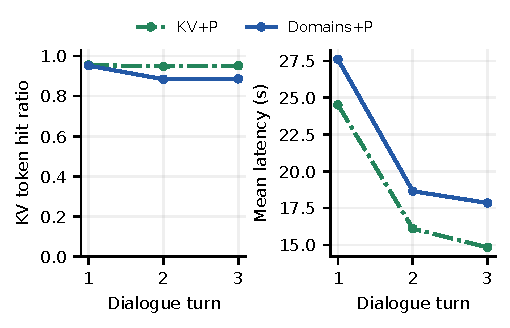
\includegraphics[width=\columnwidth]{figures/dialogue-turns.pdf}
\caption{First HTTP/2 dialogue trial. Only the first turn uses cohort preparation.
Later turns expose a cache-locality cost under Domains+P. The lower full-rollout
latency does not imply lower mean latency at each turn.}\label{fig:turns}
\end{figure}

\begin{figure*}[t]\centering
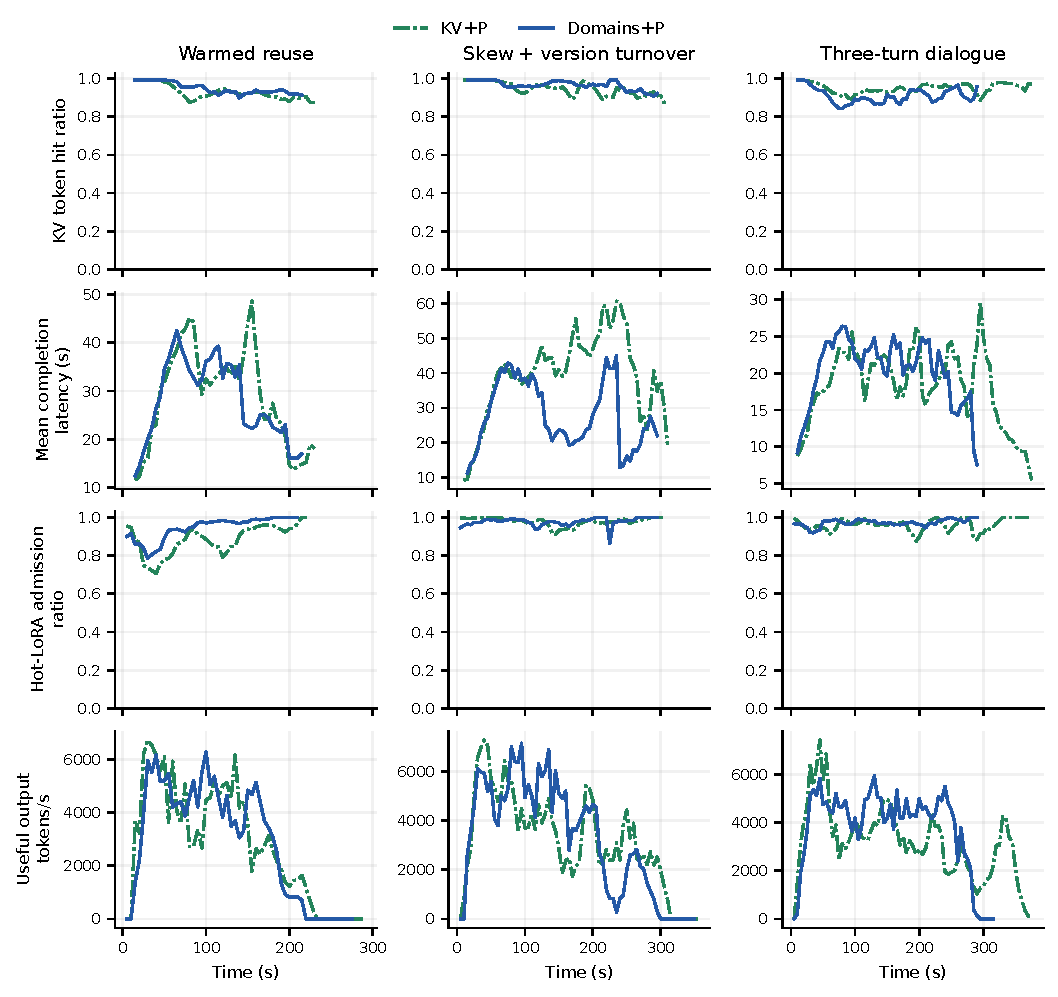
\includegraphics[width=\textwidth]{figures/time-series.pdf}
\caption{First HTTP/2 trial of each RL-shaped workload. Curves use 20-second
trailing windows sampled every five seconds. KV ratio and mean latency use
completed logical requests; hot-LoRA ratio uses interpolated engine admission
counter differences, including seeds. Useful throughput excludes seed outputs.
Windows with no relevant completions or admissions have gaps.}
\label{fig:timeseries}\end{figure*}

\begin{figure*}[t]\centering
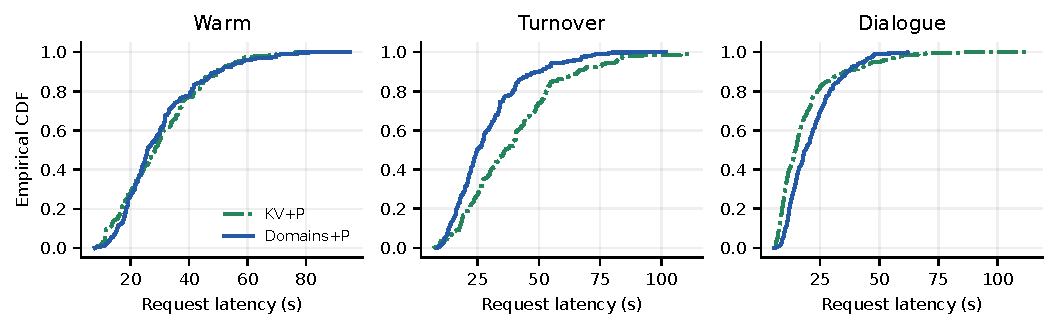
\includegraphics[width=\textwidth]{figures/request-cdf.pdf}
\caption{Individual-request latency distributions in the first HTTP/2 trials.
Each curve includes every completed logical request and any preparation time.
The samples are dependent; these CDFs are descriptive, not independent
replications.}\label{fig:cdf}\end{figure*}

\subsection{Longer generation under independent loops}
\begin{table*}[t]\centering\small\setlength{\tabcolsep}{4pt}
\begin{tabular}{llrrrrr}\toprule
Output tokens & Policy & Requests & Window completions & Window tok/s & Window mean (s) & Loads / 1k\\\midrule
512 & KV+P & 3648 & 2389 & 5097 & 71.2 & 16.4 \\
512 & Domains+P & 4160 & 2887 & 6159 & 66.5 & 23.8 \\
1,024 & KV+P & 1856 & 1068 & 9114 & 97.2 & 2.7 \\
1,024 & Domains+P & 1536 & 889 & 7586 & 106.0 & 21.5 \\
\bottomrule\end{tabular}
\caption{Longer-output controls. Window metrics use completions from 60 seconds to the arrival-window end: 300 seconds for 512-token outputs and 180 seconds for 1,024-token outputs. Admitted work drains afterward. Total work depends on policy, so loads are normalized by logical requests. Each output length has one trial.}\label{tab:long}
\end{table*}

The longer-output controls retain skewed groups and independent publication
delays. Unlike the fixed-round comparisons, clients admit new rollouts until
the same wall-clock cutoff, then drain submitted work. Faster progress changes
the number of requests and checkpoint versions encountered. Window throughput
therefore measures this closed-loop workload, not a fixed-work speedup or an
estimate of stationary engine capacity. Window latency also describes the
requests that complete in that interval, rather than all arrivals.

With 512-token outputs, Domains+P completes 2,887 requests during seconds
60--300 versus KV+P's 2,389, raising useful window throughput from 5,097 to
6,159 tokens/s (20.8\%). Across the full replay, it completes 4,160 versus
3,648 requests and achieves 5,414 versus 4,491 tokens/s (20.6\%). Mean request
latency falls from 71.31 to 62.17\,s (12.8\%), p95 from 155.49 to 137.54\,s
(11.5\%), and mean rollout time from 98.97 to 81.30\,s (17.9\%). Both arms
finish without retries. Fourteen KV+P clients and fifteen Domains+P clients
reach the second checkpoint, yielding 30 and 31 versions respectively.

The mechanism differs from the 64-version result. Busy observations with an
idle replica fall from 59.6\% to 28.1\%, while active-load variation falls from
.770 to .593. GPU loads increase from 16.4 to 23.8 per thousand logical
requests, and the seed-inclusive uncached-input fraction rises from 7.1\% to
10.5\%. The router spends more on replicated state to serve more overlapping
work. There is still substantial imbalance; these observations do not show
that every replica is saturated whenever the pool has a queue.

The 1,024-token control exposes a regression. During seconds 60--180,
Domains+P completes 889 requests versus 1,068 for KV+P: window throughput
falls from 9,114 to 7,586 tokens/s (16.8\%). Across the full replay, mean
request latency rises from 105.97 to 113.81\,s (7.4\%), p95 from 200.93 to
217.86\,s (8.4\%), and mean rollout time from 138.16 to 150.75\,s (9.1\%).
Both arms finish without retries. Busy observations with an idle replica rise
from 24.3\% to 38.5\%, and active-load variation rises from .507 to .632.
GPU loads rise from 2.7 to 21.5 per thousand logical requests; seed-inclusive
uncached input rises from 5.7\% to 9.3\%.

Full-replay throughput alone would conceal this result: it rises from 5,674
to 6,011 tokens/s (5.9\%), but Domains+P admits only 1,536 requests versus
1,856 and has a shorter drain. The fixed-window and latency measurements do
not support an improvement for this control. Only one client in each arm
reaches the next version, so it is primarily a longer-decode check, not a
broad turnover test. Each longer-output pair has one trial; the evaluation
neither attributes this regression to a single score term nor establishes
robustness across output lengths. The fixed calibration and one-batch escape
budget require further evaluation when decoding dominates.

\subsection{Why the initial policies were insufficient}
We first evaluated 512 requests from 32 adapter versions, 256 concurrent streams,
4,096-token prompts, and 128-token outputs. This pilot did not saturate the
pool's 288 running slots. Table~\ref{tab:pilot} exposes a failure of optimizing
one locality metric: the first domain policy reduced GPU adapter loads from
165 to 54, but still finished 3.7\% slower than KV affinity. Unrestricted
estimated-work routing dispersed reusable prefixes and was slower still.
These are exploratory trials used to refine the design, not independent
validation runs.

\begin{table}[t]
\centering\small
\begin{tabular}{lrrrr}
\toprule
Policy & Time (s) & KV hit & Hot LoRA & Loads\\
\midrule
KV & 42.2 & .414 & .586 & 165\\
Work & 50.6 & .017 & .426 & 316\\
Basic domains & 43.8 & .368 & .885 & 54\\
\bottomrule
\end{tabular}
\caption{Exploratory 32-adapter pilot. Lower adapter traffic alone did not
improve completion time.}\label{tab:pilot}
\end{table}

The placement map also matters when the catalog approaches aggregate slot
capacity. On the actual eight-replica topology, hashing 16 model identities and
co-locating their four versions assigned between zero and 16 preferred adapters
to each host. The excess above eight slots totaled 12 adapters. Hashing the 64
exact versions independently still left ten excess assignments. The
slot-budgeted primary map removes this particular preferred-placement
imbalance. It does not prevent later demand-driven replication from exceeding
the slot budget.

\subsection{Separating preparation from routing}
A second pilot used 16 clients, two groups of 16 siblings per client, one
rollout, 8,192-token inputs, and 128-token outputs. Preparing the shared boundary
reduced KV affinity's mean latency from 15.49 to 9.68\,s and raised useful
throughput from 2,363 to 3,559 tokens/s. Domains+P achieved 9.96\,s and 3,415
tokens/s: it did not improve on the stronger baseline. Its GPU loads were lower
(14 versus 27), yet that advantage did not determine completion time.

This pilot retained the earlier 64-entry host catalog, although only 16 versions
were used during the measured burst. The final-trial reset removes that
experiment-order dependency. We retain the pilot to explain the control and
design decisions, not as a final claim about the revised reset procedure.

\subsection{Version turnover: separating three effects}
The initial HTTP/1 turnover trial completes all four arms without a retry.
Table~\ref{tab:turnover-ablation} separates prefix preparation, load-aware
placement, and adapter domains. Relative to KV, adding preparation reduces mean
request latency by 12.6\% and increases replay throughput by 22.0\%. Its visible
KV hit ratio rises from .842 to .967, but the uncached-input fraction including
seed work falls only from 15.8\% to 8.4\%. The distinction prevents auxiliary
prefill from being mistaken for free cache reuse.

Relative to KV+P, Domains+P reduces mean request latency by 27.8\%, p95 latency
by 28.1\%, and mean rollout latency by 32.3\%. Busy observations with at least one
idle replica fall from 53.1\% to 2.0\%; the mean replica-load coefficient of
variation falls from .765 to .408. These observations support the intended
mechanism: a few congested affinity destinations no longer determine most
clients' rollout time. GPU adapter loads nevertheless increase from 66 to 88,
and seed-inclusive uncached input increases from 8.4\% to 9.7\%. The improvement
comes with additional state replication.

\begin{table*}[t]\centering\small
\begin{tabular}{lrrrrrrrr}\toprule
Policy & Output tok/s & Mean request (s) & p95 (s) & Mean rollout (s) & KV hit & Loads & Registers & Busy idle\\\midrule
KV & 2,738 & 37.44 & 72.15 & 57.74 & .842 & 66 & 51 & 65.8\%\\
KV+P & 3,341 & 32.72 & 69.08 & 47.06 & .967 & 66 & 51 & 53.1\%\\
Domains+P & 3,137 & 23.63 & 49.65 & 31.84 & .971 & 88 & 57 & 2.0\%\\
Work+P & 3,059 & 23.43 & 51.31 & 30.30 & .977 & 144 & 83 & 5.3\%\\
\bottomrule\end{tabular}
\caption{Initial version-turnover ablation: 4,352 requests per arm, 8,192 input
and 256 output tokens, eight H200 replicas, HTTP/1, no retries. Busy idle is the
fraction of sampled observations with at least 288 active requests and an idle
replica. This single trial is separate from the HTTP/2 comparisons.}
\label{tab:turnover-ablation}\end{table*}

\begin{figure*}[t]\centering
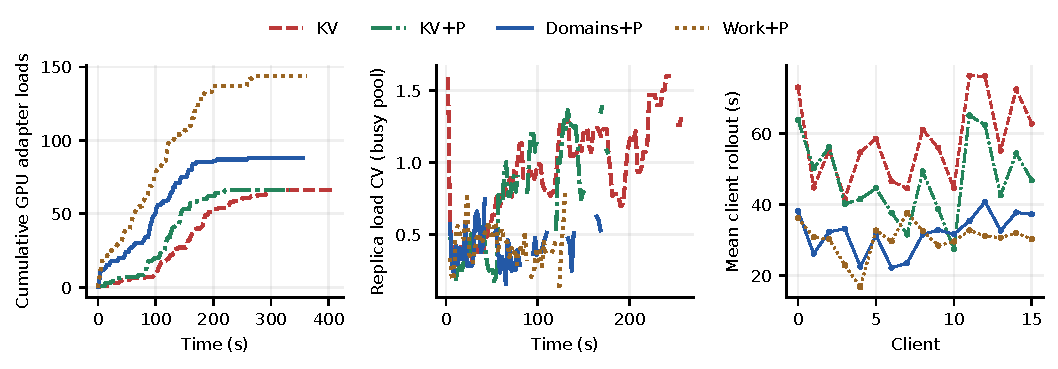
\includegraphics[width=\textwidth]{figures/turnover-mechanisms.pdf}
\caption{Initial turnover ablation. Left: cumulative GPU adapter loads. Middle:
replica-load variation when the pool has at least 288 active requests. Gaps omit
less-loaded periods. Right: each independent client's mean rollout time.
Load-aware placement improves balance; domain restriction reduces adapter
movement relative to unrestricted work routing.}\label{fig:mechanisms}
\end{figure*}

\paragraph{Why replay throughput can still decrease.}
Despite lower average latencies, Domains+P takes 355.1\,s versus KV+P's
333.5\,s, reducing replay throughput by 6.1\%. Client 15's initial rollout
takes 58.8\,s under Domains+P versus 33.5\,s under KV+P. Its later rollouts are
faster under Domains+P, but three approximately 96\,s overlapping update
intervals preserve the initial delay on the replay's critical path. The experiment
therefore demonstrates an average-latency improvement, not a training-throughput
improvement. A scheduler optimizing total work does not directly optimize each
independent training loop's completion time.

\paragraph{What the adapter domains contribute.}
Work+P has a similar mean request latency (23.43\,s versus 23.63\,s), while
Domains+P reduces GPU loads by 38.9\% (144 to 88) and registration calls by
31.3\% (83 to 57). Summed host elapsed loading time falls from 9.68 to
6.01\,s, not an additive 3.67\,s wall-clock saving. The evidence attributes much
of the latency improvement to load-aware placement and a separate reduction in
state movement to domains. It does not establish that minimizing loads alone
maximizes throughput.

\paragraph{Cache observation and preparation audit.}
Before this trial, all 72 problem groups in every arm have a reported reusable
7,168-token prefix. Missing initial cache observations therefore do not explain
the baseline comparison. Preparation also does not guarantee permanent reuse.
KV+P has 976 sibling requests with less than the prepared 8,128-token match;
all execute on their seed's replica, and 832 retain exactly the 7,168-token
prefix. Domains+P has 758 such requests, 730 on the seed's replica. Most observed
losses cannot be explained by routing to a different host. Cache eviction and
the hybrid engine's reusable-boundary behavior remain relevant after placement.

\subsection{Routing overhead}
The initial turnover run measures a 136\,$\mu$s p95 domain-selection duration
and a 1.48\,ms p95 engine snapshot duration. The mean serialized routing-state
size is approximately 8.1\,KB per replica, excluding the additional counters
collected by the benchmark observer. These measurements exclude network polling
from the synchronous selection duration; they do not imply zero control-plane
cost.

An isolated CPU benchmark uses 64 catalog entries, 36 observed requests per
replica, 128 local reservations, 8,192-token prompts, 200 warmup calls, and
1,000 measured selections. On an Intel Xeon Platinum 8375C, domain selection for
single requests has p95 costs of 150, 449, and 1,713\,$\mu$s at 8, 32, and 128
replicas. Groups of eight amortize the mean cost to 28, 68, and 252\,$\mu$s per
sibling; their p95 still includes new chunk planning. Prefix hashing separately
has a 174\,$\mu$s median in this environment. These are CPU cost measurements,
not distributed scalability experiments.

For 64 adapters, rebuilding the preferred map costs 89, 236, and
747\,$\mu$s at p95 for the same replica counts when the topology's hash orders
are retained; rebuilding those orders raises the figures to 213, 710, and
2,864\,$\mu$s. The cached map avoids that work on ordinary selections. Polling
still scales with frontend count times replica count.

\subsection{Transport-affected stress results}
The HTTP/1 64-version stress pilot uses 1,024 streams and 3,072 generations.
KV takes 533.8\,s with 202 retries; the intermediate balanced-domain policy
takes 410.0\,s with 109 retries. The apparent throughput improvement is 30.2\%,
while mean request latency increases from 84.9 to 86.8\,s. This result is
retained as a stress observation, not a clean estimate of the final policy's
routing benefit. The prototype and the retry workload both differ.

The initial warmed HTTP/1 KV and KV+P arms take 551.3 and 574.9\,s with one
and three retries respectively. In one traced failure, the request disappears
from engine observations approximately 293\,s before its HTTP read fails;
increasing the client timeout to 600\,s does not remove the roughly 360\,s
failure. These observations motivate the separate transport phase, not removal
of failed attempts from the metric denominator. The unfinished domain arm is
canceled and is not reported as a completed trial.

The single-client HTTP/2 diagnostic completes 2,048 default-policy requests in
719.5\,s, with no retries but only 1.6\% KV hits and 2,354 GPU loads. Its mean
request latency is 157.4\,s, while mean backend latency is 24.4\,s. Only nine
complete pool observations return during the run. The verified 100-stream
client cap and shared observer connection invalidate a pool-saturation claim
for this configuration. The corrected general-serving comparison changes the
client topology for every policy and is reported separately.
